\section{Experiments}
\label{sec:experiments}
In order to evaluate the proposed approach, we answer two questions related to two laws of RTE \cite{foster_combinators_2007}. 

\tb{RQ1}: A state machine \ti{sm} is used for generating code. The generated code is reversed by the backward transformation to produce another state machine \ti{sm'}. Are \ti{sm} and \ti{sm'} identical? In other words: whether the code generated from UML state machines model can be used for reconstructing the original model.

\tb{RQ2}: A state machine \ti{sm} is used for generating code. The generated code is modified by adding/deleting/modifying elements such as states, transitions, or events. The modified code is then reversed by merging changes to \ti{sm}. Are modifications in the modified code propagated to \ti{sm}?

This section reports our experiments targeting to the two questions. Two types of experiments are conducted. For each type, the number of elements in models are taken into account by a JAVA program. Fig. \ref{fig:EvaluationStrategyBoth} (a) and (b) show the evaluation methodologies to answer \tb{RQ1} and \tb{RQ2}, respectively. Additionally, 
%the time complexity and performance analysis of our approach is presented.
 results of a lightweight experiment on the semantic conformance of runtime execution of the generated code are also shown afterward.

\begin{figure}
\centering
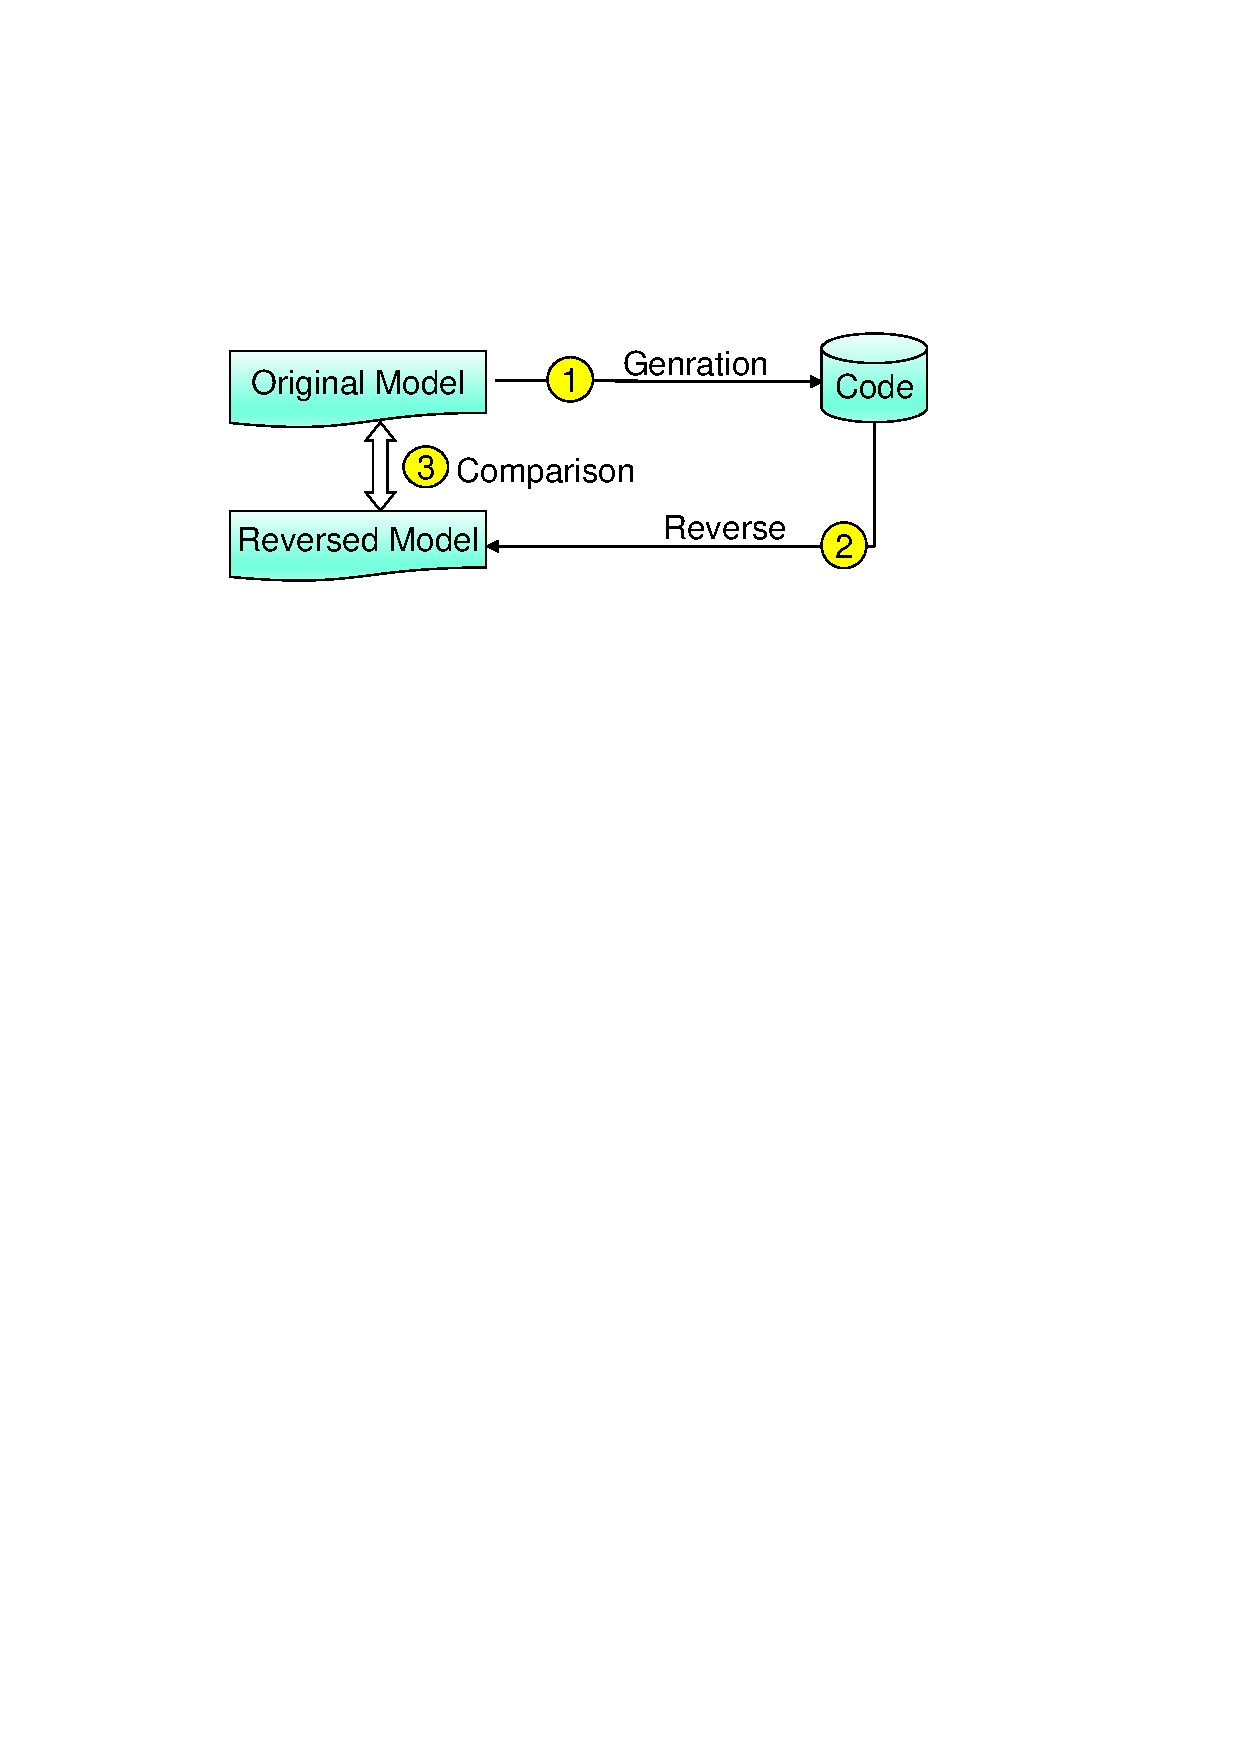
\includegraphics[clip, trim=0.8cm 17.1cm 0.3cm 4.0cm, width=0.8\columnwidth]{figures/EvaluationStrategyBoth}
\caption{Evaluation methodology to answer RQ1} 
\label{fig:EvaluationStrategyBoth}
\end{figure}

\begin{comment}
\begin{figure}
\centering
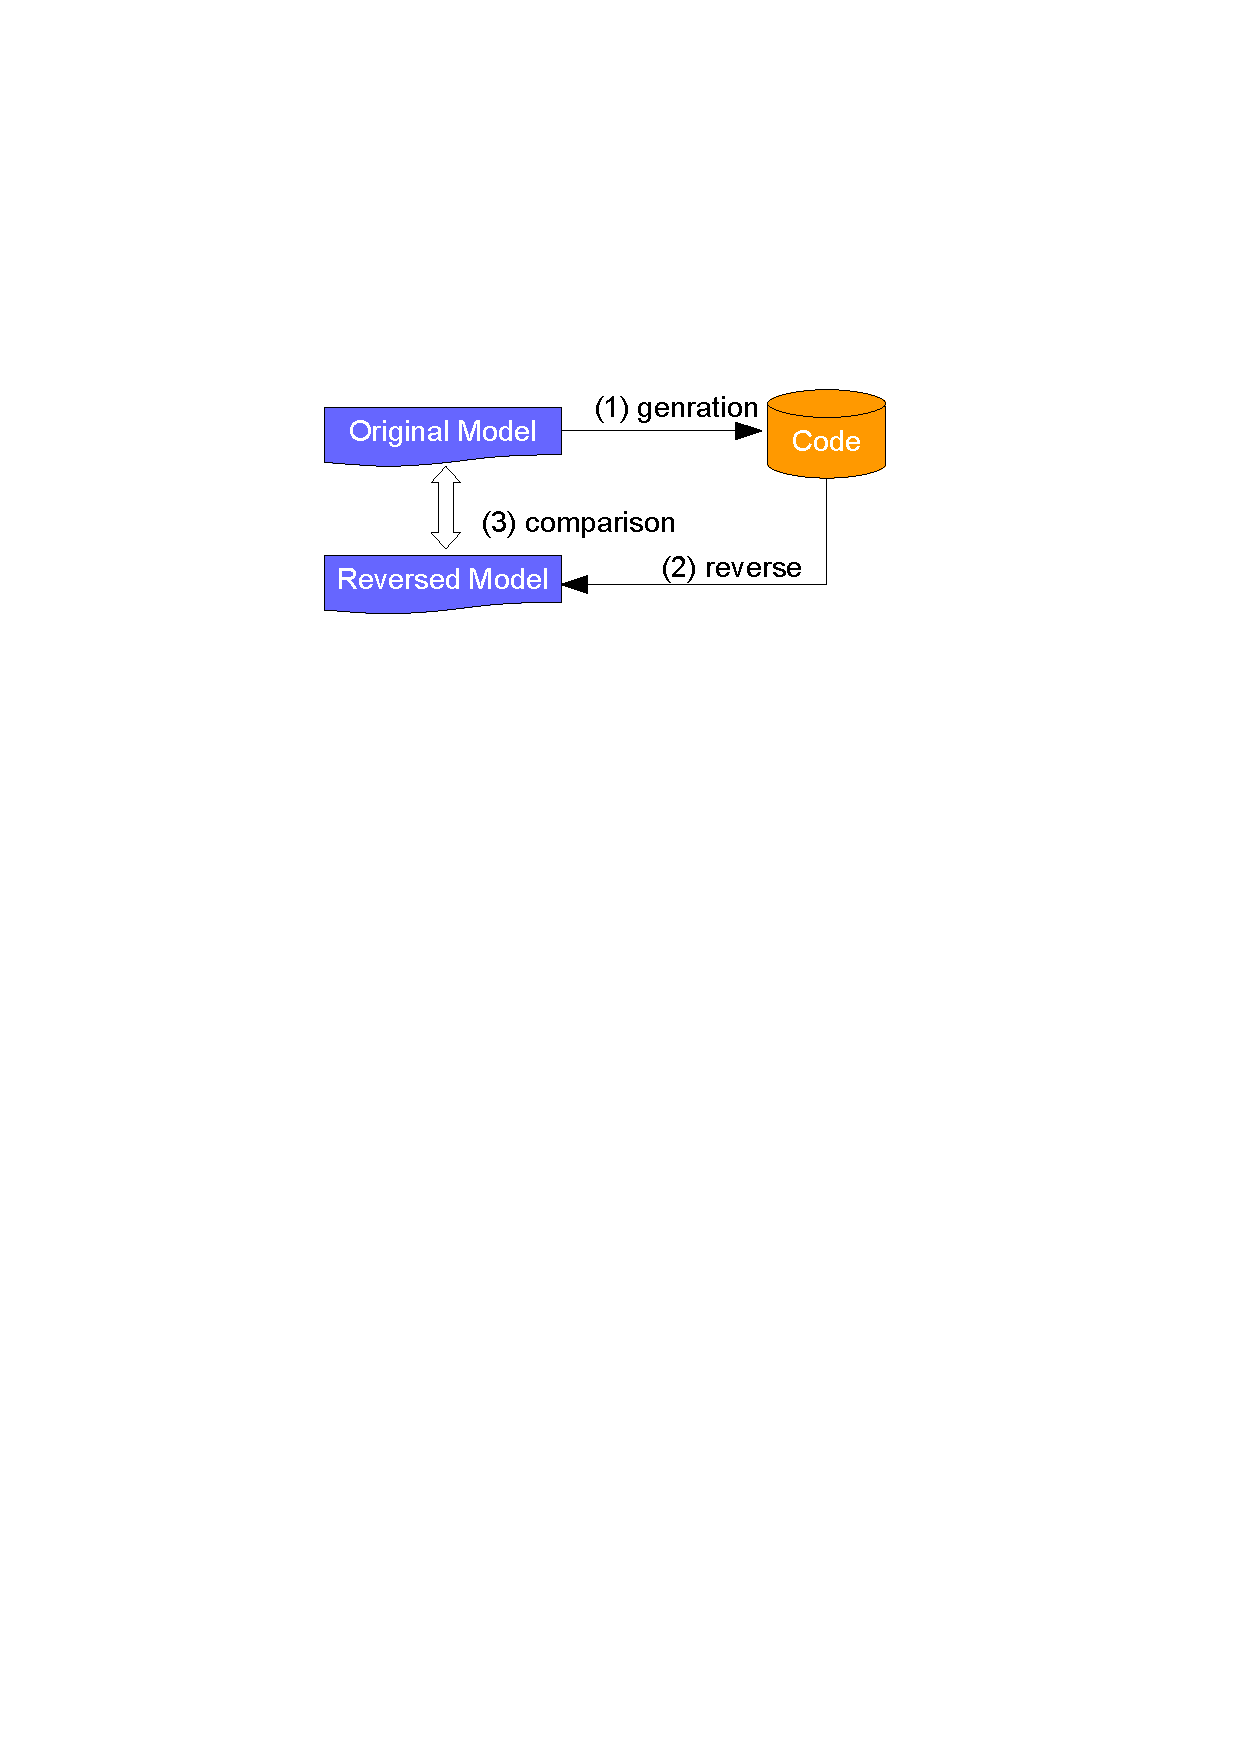
\includegraphics[clip, trim=5.5cm 19cm 5.5cm 6cm, width=0.3\textwidth]{figures/strategy1}
\caption{Evaluation methodology to answer RQ1} 
\label{fig:strategy1}
\end{figure}

\begin{figure}
\centering
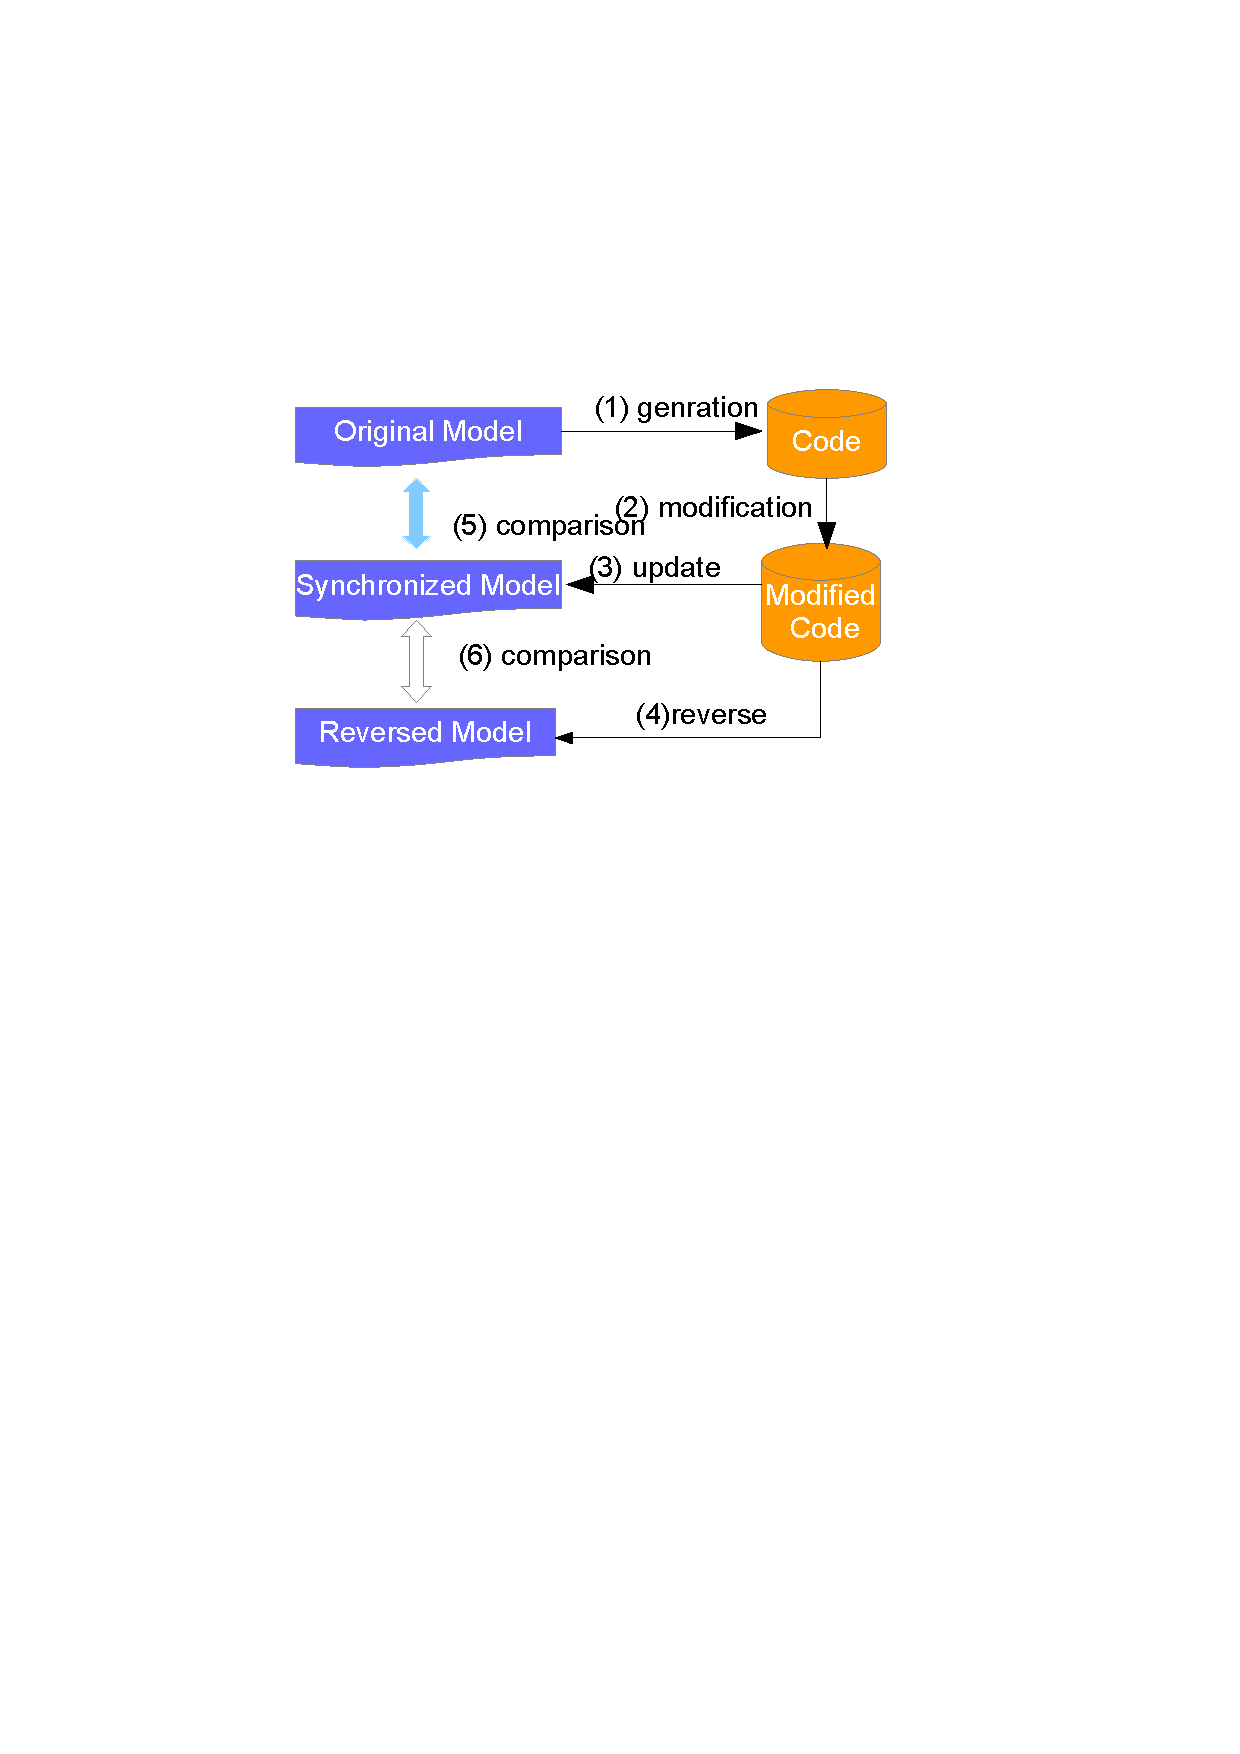
\includegraphics[clip, trim=4.5cm 16.5cm 5.5cm 6.5cm, width=0.3\textwidth]{figures/strategy2}
\caption{Evaluation methodology to answer RQ2} 
\label{fig:strategy2}
\end{figure}
\end{comment}

%Furthermore, in software development projects, some traditional programmers might want to practice with code in a traditional way and some MDE developers may prefer working with models. Therefore, it is necessary to compare the development/maintenance cost between the two practices by comparing the number of steps needed to do the same action. 


\subsection{Reversing generated code}
This experiment is targeting \tb{RQ1}. Random models containing hierarchical state machines are automatically generated by a configurable model generator. The generator can configured to generate a desired average number of each USM element type. 

For each model, a context class and its behavior described by a USM are generated. Each USM contains 80 states including atomic and composite states, more than 234 transitions. The number of lines of generated C++ code for each machine is around 13500. Names of the generated states are different. An initial pseudo state and a final state are generated for each composite state and containing state machine. Other elements such as call events, time events, transition/entry/exit actions and guards are generated with a desired configuration. For each generated call event, an operation is generated in the context class which is also generated. The duration is generated for each time event. 

\begin{comment}
\begin{table}
\centering
\caption{Set-up information for model generation}
\label{table:setup}
\begin{tabular}{|l|l|}
\hline
\rowcolor{Gray}
Description                                     & Value            \\ \hline
%Number of generated states                      & 80               \\ \hline
%Number of generated transitions                 & \textgreater 234 \\ \hline
Probability of having an event for transition   & 0.8              \\ \hline
Probability of having CallEvent for transition  & 0.7              \\ \hline
Probability of having an entry/exit action for state & 0.7              \\ \hline
Probability of having a transition action and guard       & 0.7              \\ \hline
\end{tabular}
\end{table}
\end{comment}

%The set up information for the USM generation is shown in Table \ref{table:setup}. 
The procedure for this experiment, for each original UML model containing a state machine, consists of 3 steps: (1) code is generated from an \tb{original model}, (2) the generated code is reversed to a \tb{reversed model}, and (3) the latter is then compared to the \tb{original state machine} by using information of USM such as the numbers of states and transitions. 

\begin{table}
\centering
\caption{Three of model results of generation and reverse: Abbreviations are atomic states (AS), composite states (CS), transitions (T), call events (CE), time events (TE)}
\label{table:law1-resultat}
\begin{tabular}{|l|l|l|l|l|l|l|}
\hline
\rowcolor{Gray}
Test ID & AS & CS & T & CE & TE & Is reverse correct? \\ \hline
1       & 47 & 33 & 234 & 145 & 40 & Yes                 \\ \hline
2       & 42 & 38 & 239 & 145 & 36 & Yes                 \\ \hline
%3       & 43 & 37 & 238 & Yes                 \\ \hline
..      & .. & .. & .. & .. & .. & Yes                 \\ \hline
300       & 41 & 39 &240 & 142 & 37 & Yes                 \\ \hline
\end{tabular}
\end{table}
 
 
\begin{comment}
\begin{table*}[]
\centering
\caption{MODEL RESULTS OF GENERATION AND REVERSE}
\label{table:law1-resultat}
\begin{tabular}{|l|l|l|l|l|l|l|l|l|l|l|l|l|l|}
\hline
\rowcolor{Gray}
Test ID & AS & CS & D  & T   & EA & ExA & TA  & CE  & TE & G   & I  &    & Is reverse correct? \\ \hline
1       & 47 & 33 & 8  & 234 & 53 & 50  & 149 & 145 & 40 & 147 & 34 & 25 & Yes                 \\ \hline
2       & 42 & 38 & 8  & 239 & 52 & 59  & 165 & 145 & 36 & 133 & 39 & 31 & Yes                 \\ \hline
3       & 43 & 37 & 7  & 238 & 54 & 59  & 159 & 141 & 34 & 145 & 38 & 28 & Yes                 \\ \hline
..      & .. & .. & .. & ..  & .. & ..  & ..  & ..  & .. & ..  & .. & .. & Yes                 \\ \hline
300       & 41 & 39 & 10 & 240 & 56 & 55  & 165 & 142 & 37 & 151 & 40 & 33 & Yes                 \\ \hline
\end{tabular}
\end{table*}
\end{comment}

Table 1 shows the number of each type of elements in the randomly generated model, including the comparison results, for 3 of the 200 models created by the generator. We limited ourselves to 200 models for practical reasons

Table \ref{table:law1-resultat} shows the number of several types of elements in the generated models, including the comparison results, for 3 of the 300 models created by the generator. We limited ourselves to 300 models for practical reasons. No differences were found during model comparison. The results of this experiment show that the proposed approach and the implementation can successfully do code generation from state machines and reverse. 

%\subsection{Change propagation} 
We manually created two state machines (model level): one describing Java Thread life-cycle \cite{_java_thread} and the other one representing a telephone presented in \cite{Specification2007}. For each SM code is generated. Code is then manually modified. Each modification test consists of one or several actions described in Table \ref{table:cost}. The original SM is updated by doing a backward process from the modified generated code with the presence of the intermediate and original model. The updated SM ($sm_{updated}$) is in turn compared with the SM created ($sm_{reversed}$) by the reverse engineering (see Fig. \ref{fig:EvaluationStrategyBoth}). A modification test is passed if the corresponding models $sm_{updated}$ and $sm_{reversed}$ are the same. Table \ref{table:change-propa} shows the number of test cases (Tests) applied to each model, of passed test cases (Passed tests) and the result of change propagation experiment. The table shows that our approach is able to update the original state machine following code-side modifications. 

\begin{table}
\centering
\caption{Change propagation experimental results}
\label{table:change-propa}
\begin{tabular}{|l|l|l|p{3.4cm}|}
\hline
\rowcolor{Gray}
State machine & Tests & Passed tests & Is change propagation passed? \\ \hline
Java Thread       &    20     &    20      &     Yes             \\ \hline
Telephone       &   30      &     30     &      Yes       \\ \hline
\end{tabular}
\end{table}

%\subsection{Time complexity and performance}
%We are interested in knowing which element type among state, transition and event dominates the running time of the reverse engineering in case of creating new SM from code. 
To analyze the time complexity, we consider two tasks: semantic verification and SM construction from the verification output. 
%Let us use the following parameters of the input SM used in code generation: $n_{s}$ = number of states, $n_{t}$ = number of transitions, $n_{ce}$ = number of call events, $n_{te}$ = number of time events, $n_{a}$ = number of actions and guards including entry/exit/transition actions and guards which are all implemented in the context class. 

For each state, the semantic verification consists of the following phases: (1) detecting composite/sub-state pattern, (2) loop over all methods of a state class, (3) detecting entry action pattern, (4) detecting exit action pattern, (5) detecting processing \ti{CallEvent}, (6) detecting processing \ti{TimeEvent}, and (7) detecting default state pattern. 
\begin{comment}
\begin{itemize}
  \item Detecting composite/sub-state pattern: $C_{childParentPattern} = ns^2 = O (ns^2)$.
  \item Loop over all methods of a state class: $CfindAllStateOperation = ns + nce + nt$. 
  \item Detecting entry action pattern: $Centry = na + CverifyTransition + CfindFunctionDefinition 
      = 6ns + 6nce + 5na + nt$
   \item Detecting exit action pattern: Cexit = 3nce + 3ns + 3na + nt
   \item Detecting processing CallEvent: CprocessEvent = 7nce + 6ns + 2nt + 2na 
   \item Detecting processing TimeEvent: CprocessTimeEvent = 6nce + 6ns + 2nt + 2na
   \item Detecting default state pattern: CsetInitDefaultState = 3nce + 3ns + nt + na
\end{itemize}

\begin{itemize}
  \item Detecting composite/sub-state pattern
  \item Loop over all methods of a state class
  \item Detecting entry action pattern
   \item Detecting exit action pattern
   \item Detecting processing \ti{CallEvent}
   \item Detecting processing \ti{TimeEvent}
   \item Detecting default state pattern
\end{itemize}
\end{comment}

Due to the space limitation, we cannot present the detail of the complexity of each phase. To sum up, the semantic verification has a worst-case complexity (abbreviations $n_{s}$, $n_{t}$, $n_{ce}$, $n_{a}$ are the number of states, transitions, call events and actions, respectively) $C_{1} = n_{s}(n_{s^2} + 9n_{t^2} + 6n_{t}n_{s} + 2n_{a}n_{ce}) = O (n_{s^3}) + O (n_{t}n_{s^2}) + O (n_{s}n_{t^2}) = O (n^3)$ with $n = max (n_{t}, n_{s})$. The worst-case occurs if a state can accept all incoming events, all transitions have the same source state and all states contain each other. This case is unrealistic.

The SM construction from the verification output has a worst-case time complexity $C_{2} = O (n_{s^2}) + O (n_{s} n_{t}) = O (n_{^2})$. Therefore, the reverse engineering has a worst-case complexity of $O (n^3)$ with $n = max (n_{s}, n_{t})$.

To analyze the performance of reverse engineering, we randomly generate 5 models with base set up information in which the numbers of states and transitions are 20 and 50, respectively. We use a Dell Latitude E554 laptop with a 2.1GHz Intel Core i7 with 16 Gb of RAM. The running time of the reverse for the generated code associated with these models is measured. To analyze the impact of state and transition to the reverse performance, 
%we change the set up information by increasing either the number of states or transitions, and keep intact the other. 
we increase the number of states and transitions by five, alternatively. The models resulting from the increase are used for generating code. The running time of reverse engineering the new generated code is measured. For each measurement, three times are computed, the median of these measured values are retained. 

\begin{comment}
\begin{table}
\centering
\caption{Time measurements}
\label{table:time-measurment}
\begin{tabular}{|l|l|l|}
\hline
\rowcolor{Gray}
Increase of the number of instances  & State  & Transition \\ \hline
5            & 78021  & 62271      \\ \hline
10           & 83025  & 68374      \\ \hline
15           & 96761  & 64176      \\ \hline
20           & 118879 & 71728      \\ \hline
25           & 132763 & 73445      \\ \hline
%30           & 153120 & 75314      \\ \hline
%35           & 163538 & 78647      \\ \hline
%40           & 185361 & 81547      \\ \hline
\end{tabular}
\end{table}
\end{comment}

%Table \ref{table:time-measurment} shows the increase of the number of instances for states and transitions, and the execution time in millisecond for reversing the resulting models obtained by increasing the number of instances. 
Fig. \ref{fig:graph} shows the increase of the number of instances for states and transitions, and the increase time rate, which is the execution time for reversing modified models divided by the execution time for reversing the original model. The median execution time for reversing the original model is 64557 ms. The results show that the number of states has a higher performance impact than the number of transitions. %Fig. \ref{fig:graph} (the increase time rate is the execution time for reversing modified models divided by the execution time for reversing the original model) shows the performance comparison between the execution time for reversing the original model and the models modified by adding states and transitions. 
When the number of added states grows, the running time for reverse also grows quickly. Whereas, in case of transitions, the difference is small and not clear as we analyze that the worst-case complexity never occurs.

%Fig. \ref{fig:graph} (the increase time rate is the execution time for reversing modified models divided by the execution time for reversing the original model) also shows the performance comparison between the execution time for reversing the original model and the models modified by adding states and transitions. When the number of added states grows, the running time for reverse also grows quickly. Whereas, in case of transitions, the difference is small and not clear as we analyze that the worst-case complexity never occurs.

\begin{figure}
\centering
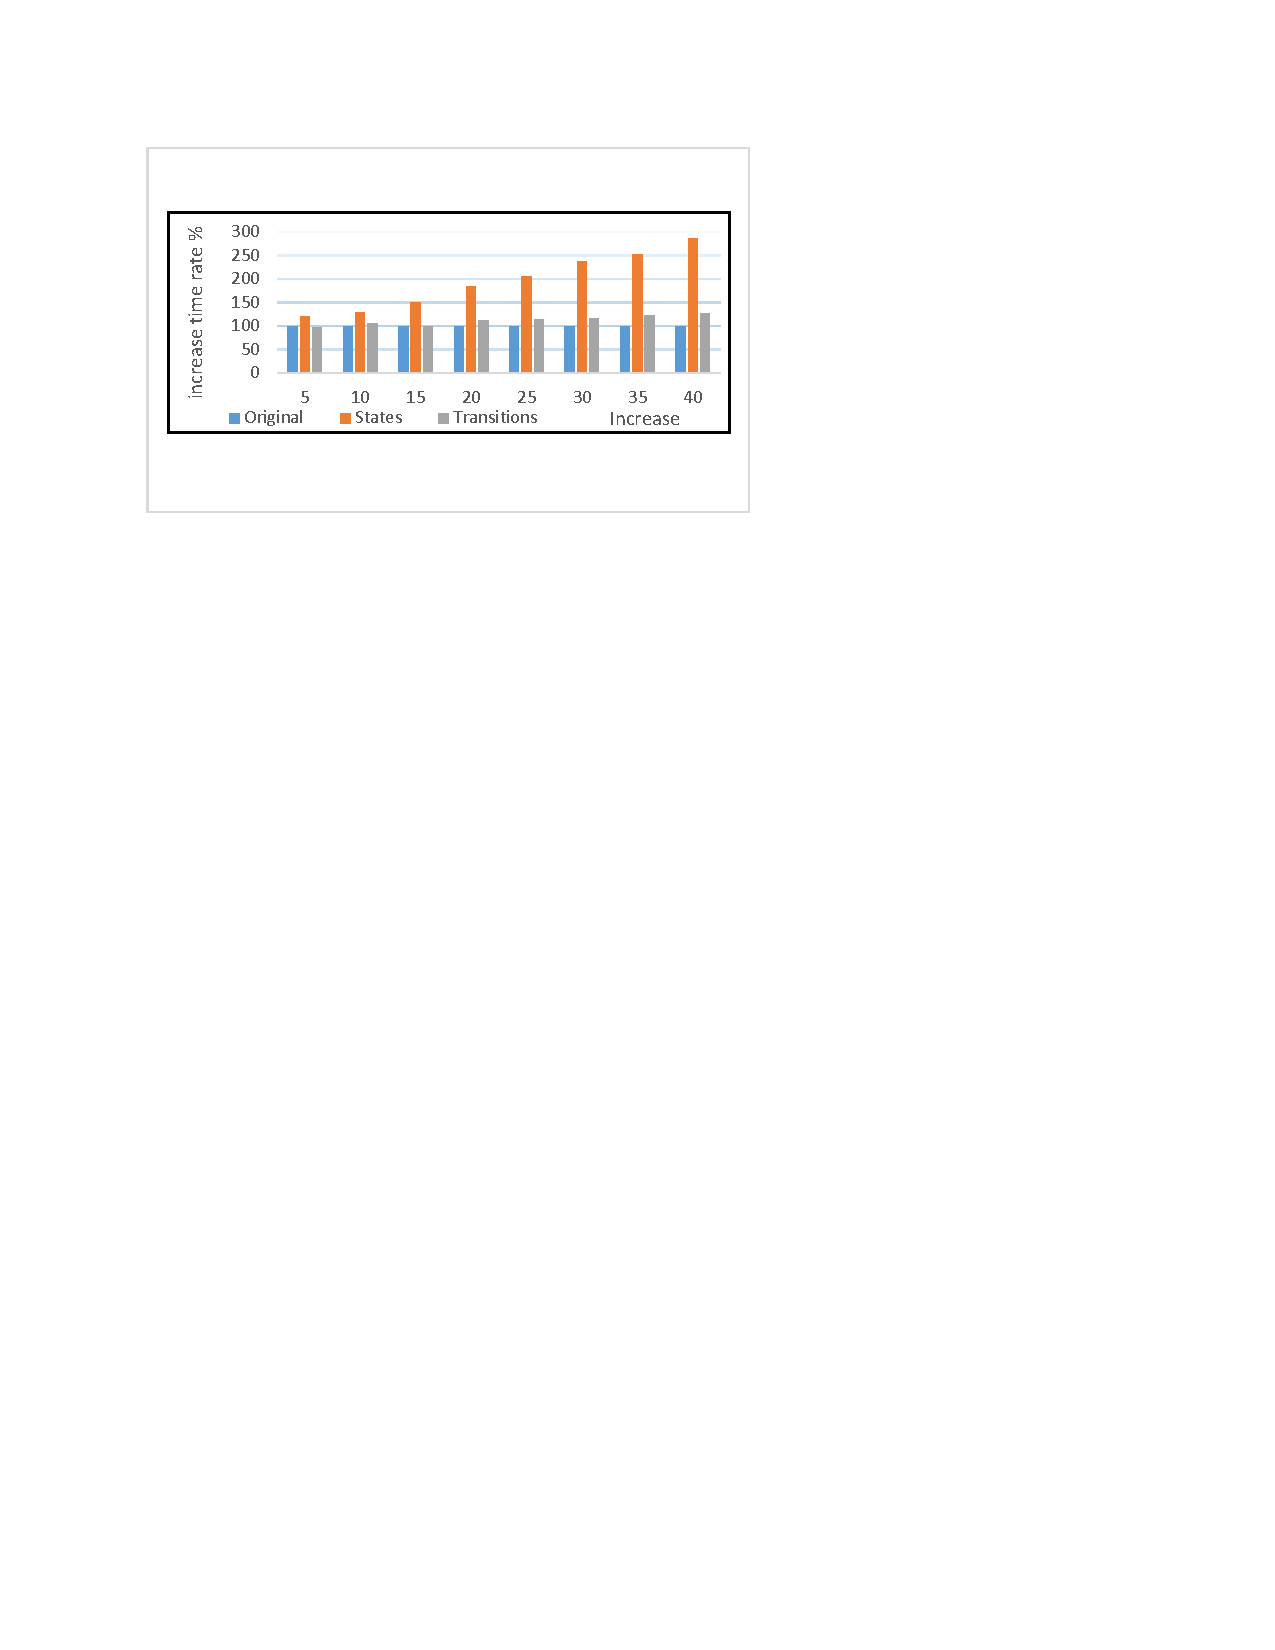
\includegraphics[clip, trim=2.8cm 20.6cm 9cm 3.6cm, width=0.35\textwidth]{figures/graph}
\caption{Performance impact comparison between states and transitions} 
\label{fig:graph}
\end{figure}

\subsection{Semantic conformance of runtime execution}
\paragraph{Bisimulation for semantic-conformance}
To evaluate the semantic conformance of runtime execution of generated code, we use a set of examples provided by Moka \cite{moka}. Moka is a model execution engine offering Precise Semantics of UML Composite Structures \cite{OMG2015}. Fig. \ref{fig:semanticconformance} shows our method. We first use our code generator to generate code (Step (1)) from the Moka example set. Step (2) simulates the examples by using Moka to extract the sequence (\ti{SimTraces}) of observed traces including executed actions. The sequence (\ti{RTTraces}) of traces is also obtained by the runtime execution of the code generated from the same state machine in a Step (3). The generated code is semantic-conformant if the sequences of traces are the same for both of the state machine and generated code \cite{Blech2005}. 

Within our scope as previously defined 30 examples of the Moka example set are tested. \ti{SimTraces} and \ti{RTTraces} for each case are the same. After experimenting with our code generator, we compare our results to the observed traces obtained by executing code generated by IBM Rhapsody \cite{ibm_rhapsody}. We find that the traces of IBM Rhapsody are not UML-compliant in some cases. Specifically, Rhapsody does not support self-triggerless transitions as in Fig. \ref{fig:autotransition} and its support for processing events is not totally semantically correct. In Fig. \ref{fig:autotransition}, right after the \ti{doActivity} action of \ti{Incrementing} finishes, the effect of \ti{T3} should be executed 5 times consecutively before the effect of \ti{T4} is automatically taken into account. In Fig. \ref{fig:Deferred}, assuming that there is an event \ti{Continue} incoming to the state machine which has a configuration \ti{(S1, S11, S21)} as current active states. While, according to the UML specification, the next configuration should be \ti{(S1, S11, final state)} and \ti{T22Effect} of the transition \ti{T22} should be executed. This means that the incoming event should be processed by the inner states of the active composite/concurrent state if the inner states accept it, otherwise the parent state does. But in case of Rhapsody the next configuration is \ti{End}.   

\begin{figure}
\centering
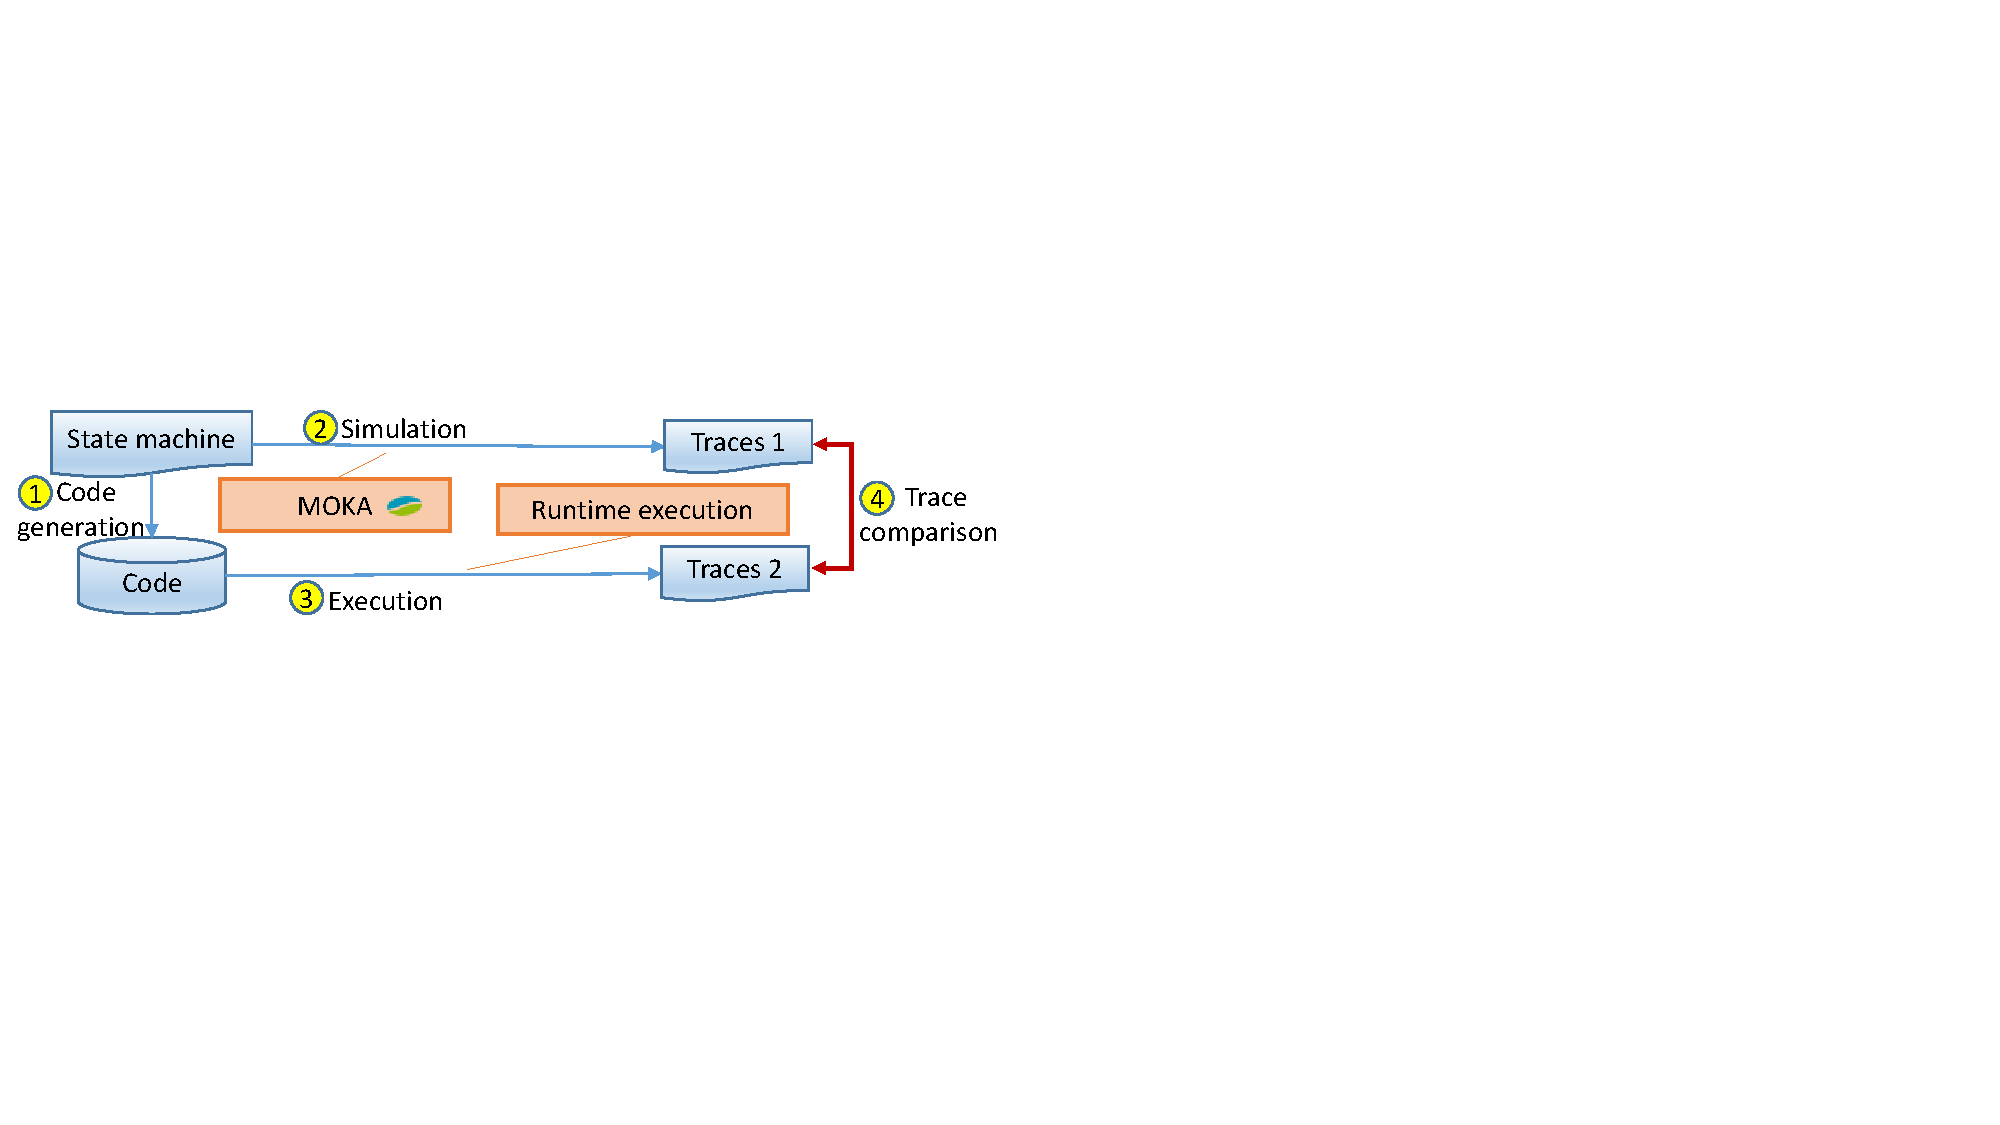
\includegraphics[clip, trim=0.8cm 8.1cm 19.4cm 6.9cm, width=\columnwidth]{figures/semanticconformance.pdf}
\caption{Semantic conformance evaluation methodology} 
\label{fig:semanticconformance}
\end{figure}

\begin{figure}
\centering
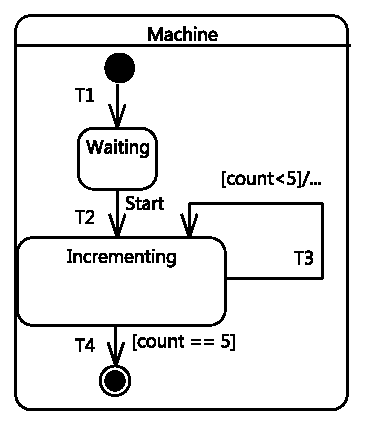
\includegraphics[clip, trim=0.25cm 0.25cm 0.25cm 0.25cm, width=0.3\columnwidth]{figures/autotransition}
\caption{Self-triggerless transition example} 
\label{fig:autotransition}
\end{figure}

\begin{figure}
\centering
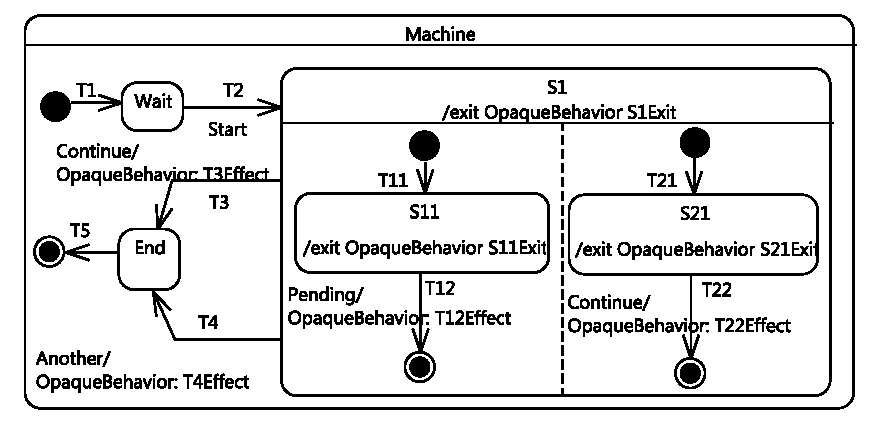
\includegraphics[clip, trim=0.25cm 0.25cm 0.25cm 0.25cm, width=0.9\columnwidth]{figures/Deferred004}
\caption{Event processing example} 
\label{fig:Deferred}
\end{figure}

\begin{comment}
\begin{figure*}
\centering
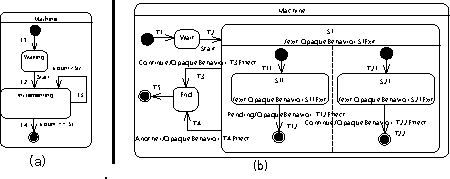
\includegraphics[width=1.5\columnwidth]{figures/ex}
\caption{Self-triggerless transition (a) and event processing (b) examples} 
\label{fig:ex}
\end{figure*}
\end{comment}

\paragraph{Finite state machine}
We evaluate the semantic-conformance of the generated code runtime execution by using deterministic finite state machines (FSMs). The latter is a mathematical model of computation and also a simplified version of UML state machine. In this experiment, we use FSMs for recognizing input symbols. Each FSM contains numerous states. The active state of the FSM can be changed following the acceptance of an input symbol. Fig. \ref{fig:fsm} shows our method to experiment. For each FSM, we create an equivalent UML state machine. Each input symbol of the FSM is considered as an event of the UML state machine. We use the FSM simulator in \cite{fsmsim} to generate and simulate FSMs. For each FSM, a list of observed states is recorded as output (\ti{out1}) of the simulation for each symbol list. The latter is also the input of the generated code runtime execution of the equivalent UML state machine which produces an output \ti{out2}. We then compare \ti{out1} and \ti{out2}.

We limit the number of FSMs to 20 and the number of symbol list for each FSM to 30 for practical concerns. 600 sequences of states obtained by the simulation and a same number of sequences taken by the runtime execution are respectively compared and equal. This results that our code generation approach produces semantic-conformant code in case of FSM.

\begin{figure}
	\centering
	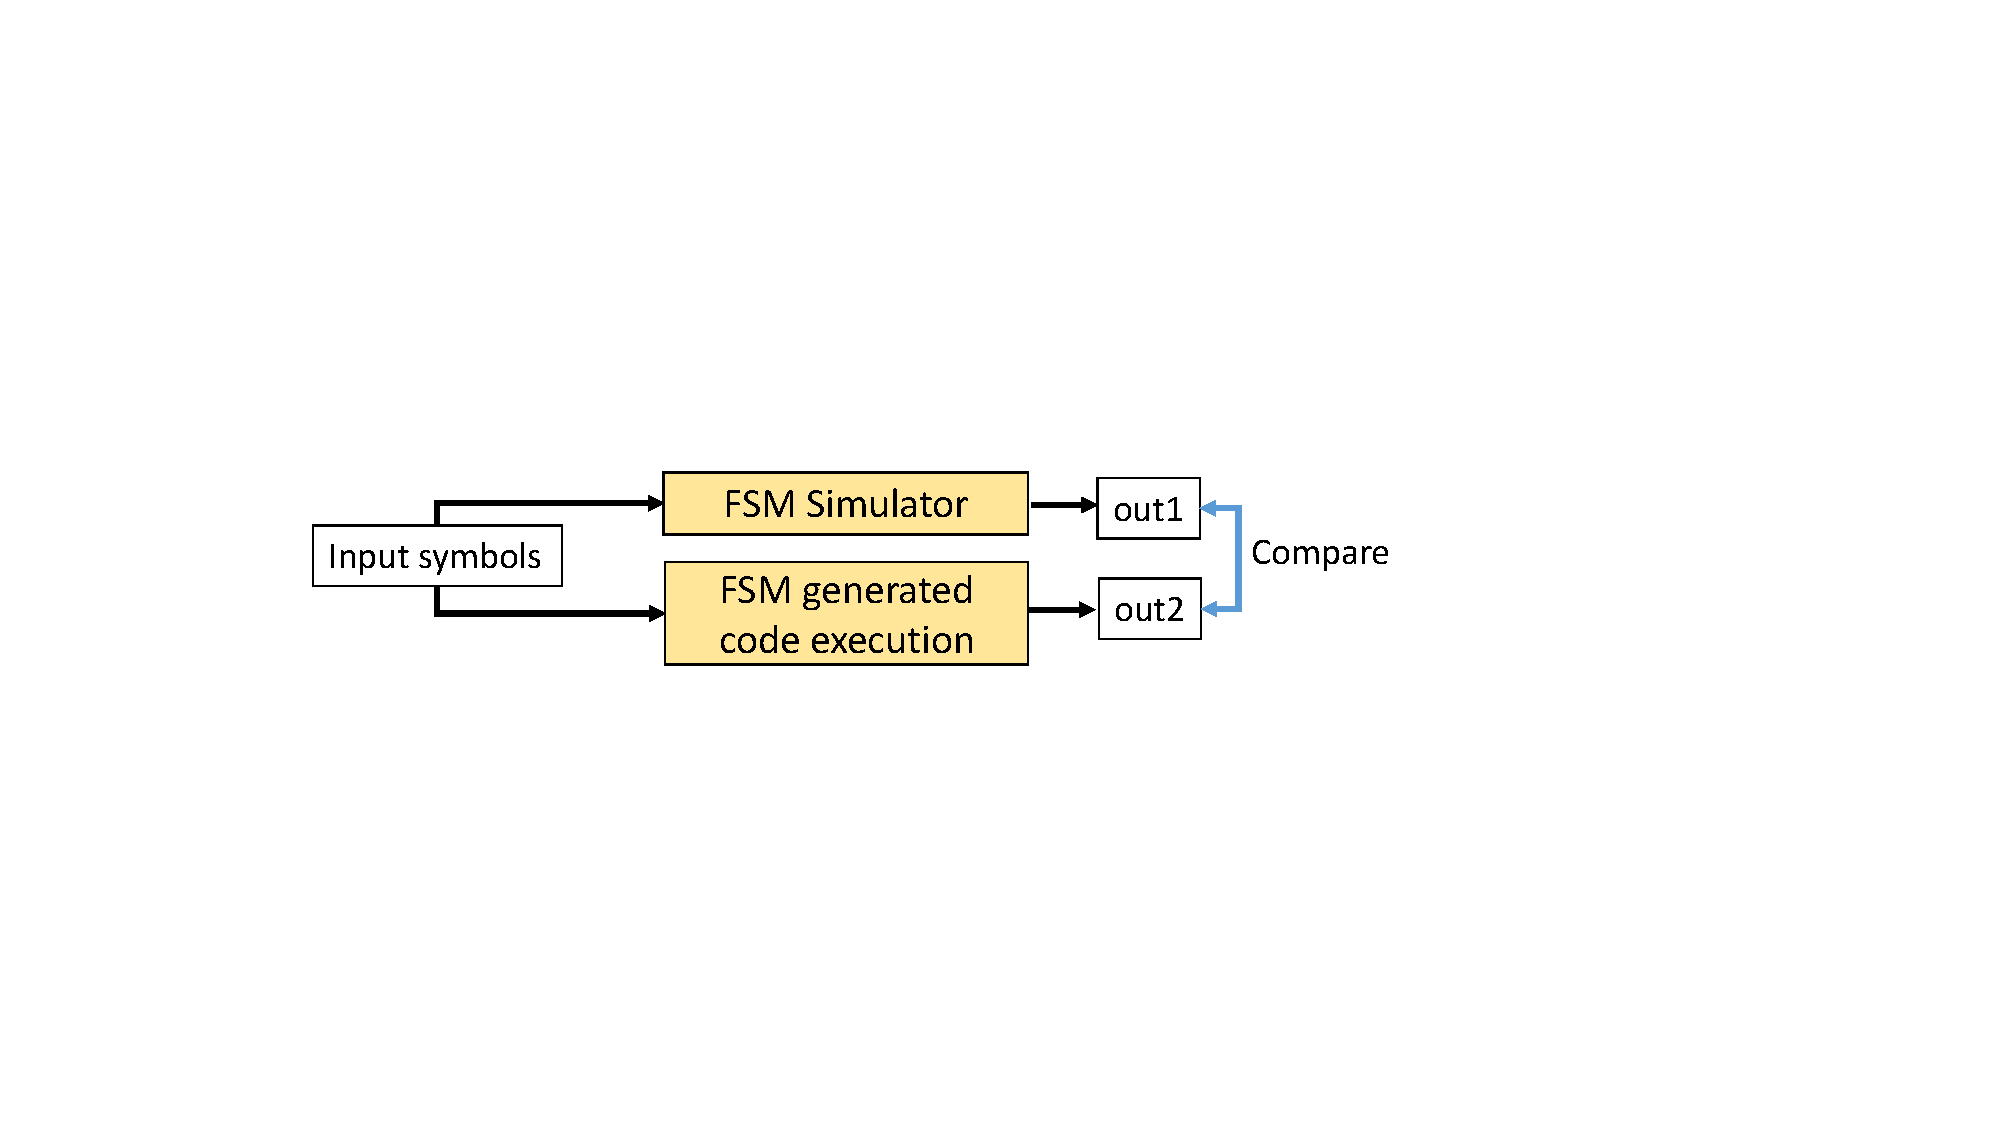
\includegraphics[clip, trim=6.5cm 7.3cm 10.25cm 7.7cm, width=0.85\columnwidth]{figures/fsm}
	\caption{FSM experiment method} 
	\label{fig:fsm}
\end{figure}

\paragraph{Comparison with IBM Rhapsody}

\subsection{Development/maintenance cost}
\label{subsec:cost}
To compare the development/maintenance cost, we investigate steps need to be done in generated code and models, respectively, to do semantically equivalents. For example, to add a state, on one hand, one step needed in USM diagrams is \ti{dragging \& dropping the state notation to the appropriate parent}. On the other hand, three code modifications are (1) \ti{create a state class inheriting from the base state and its constructors}, (2) \ti{add to the parent state class an attribute}, and (3) \ti{add a line of code to initialize the state attribute in the parent state constructor}. Table \ref{table:cost} shows the number of steps needed for each operation. In this table, model manipulations are the winner in most of cases due to graphical representation advantages but code manipulations are still useful and comparable.

\begin{table}
\centering
\caption{Cost comparison}
\label{table:cost}
\begin{tabular}{|l|l|l|}
\hline
\rowcolor{Gray}
Description                                     & Model & Code \\ \hline
Add a state                                     & 1     & 3    \\ \hline
Add a transition                                & 1     & 3    \\ \hline
Add entry/exit action                           & 2     & 2    \\ \hline
Add transition action (effect) or guard                           & 2     & 2    \\ \hline
Update action/guard                                   & 1     & 1    \\ \hline
Redirect target state of a transition           & 1     & 1    \\ \hline
Create a call event to a transition & 3     & 6    \\ \hline
Create a time event to a transition & 3     & 5    \\ \hline
Delete a state                                  & 1     & 2    \\ \hline
Delete a transition                             & 1     & 3    \\ \hline
Delete entry/exit action                        & 1     & 2    \\ \hline
Delete transition action                        & 1     & 2    \\ \hline
Delete a call event                             & 2     & many \\ \hline
Delete a time event                             & 2     & many \\ \hline
\end{tabular}
\end{table}

In software development, programmers might modify the generated code, the modifications might violate structures of code or USM semantics. To resolve this issue, as previously described, we provide a semantic analysis that partly and loosely inspects the AST of generated code. This inspection approach always reverses the code to the USM as well as the code is state machine-compliant even though the code is not compiled. This approach is very useful in practice in which programmers might partly modify code, automatically update the original USM by our RTE, and automatically re-generate state machine-compliant code. This re-generation does no more than completing missing elements in code meaning that all previous changes are preserved. This practice is also limitedly supported by Fujaba \cite{KNNZ99_2_ag} in which activity and collaboration diagrams are partly synchronized with JAVA.



